%%
%% This is file `example-1.tex',
%% generated with the docstrip utility.
%%
%% The original source files were:
%%
%% drexel-thesis.dtx  (with options: `example-part')
%% 
%% This is a generated file.
%% 
%% Copyright (C) 2010 W. Trevor King
%% 
%% This file may be distributed and/or modified under the conditions of
%% the LaTeX Project Public License, either version 1.3 of this license
%% or (at your option) any later version.  The latest version of this
%% license is in:
%% 
%%    http://www.latex-project.org/lppl.txt
%% 
%% and version 1.3 or later is part of all distributions of LaTeX version
%% 2003/06/01 or later.
%% 

\chapter{Traveling waves in other low-dimensional neuronal systems}

\section{Ensembles of minicolumns}
In section 3.2 we showed that as SCE grow in the X or Y dimension the wave speed increases due to the increased connectivity, but when the average number of connections per neuron were held constant the wave speed was constant.
We further examine these thicker, but still quasi one-dimensional SCE by examining the firing activity of purely one-dimensional sub-columns within the larger SCE (with topology 2x2x100 extracted from the central core of the thicker SCE, away from the surfaces, except of course for the 2x2 and 3x3 SCEs).
With the average number of connections held constant, the sub-columns within the larger SCE show similar firing fraction with $K$ regardless of the overall topology (Figure \ref{fig:LargeSCESubcolumns}).
We remark that as the X and Y extents increase, the behavior seems to change from traveling waves to more synchronized firing activity.
This behavior as a function of width suggests that the system dynamics transition from supporting traveling waves to a system that exhibits global synchrony.
\begin{figure}[!htb]
 \caption{ Spike raster plots for complete SCE (A) and one-dimensional sub-columns (B) for different topologies show similar firing patterns in the sub-columns regardless  of topology. 
           The wave firing fraction (C) measured within the sub-columns show the same dependence on $K$ regardless of the topology.}
   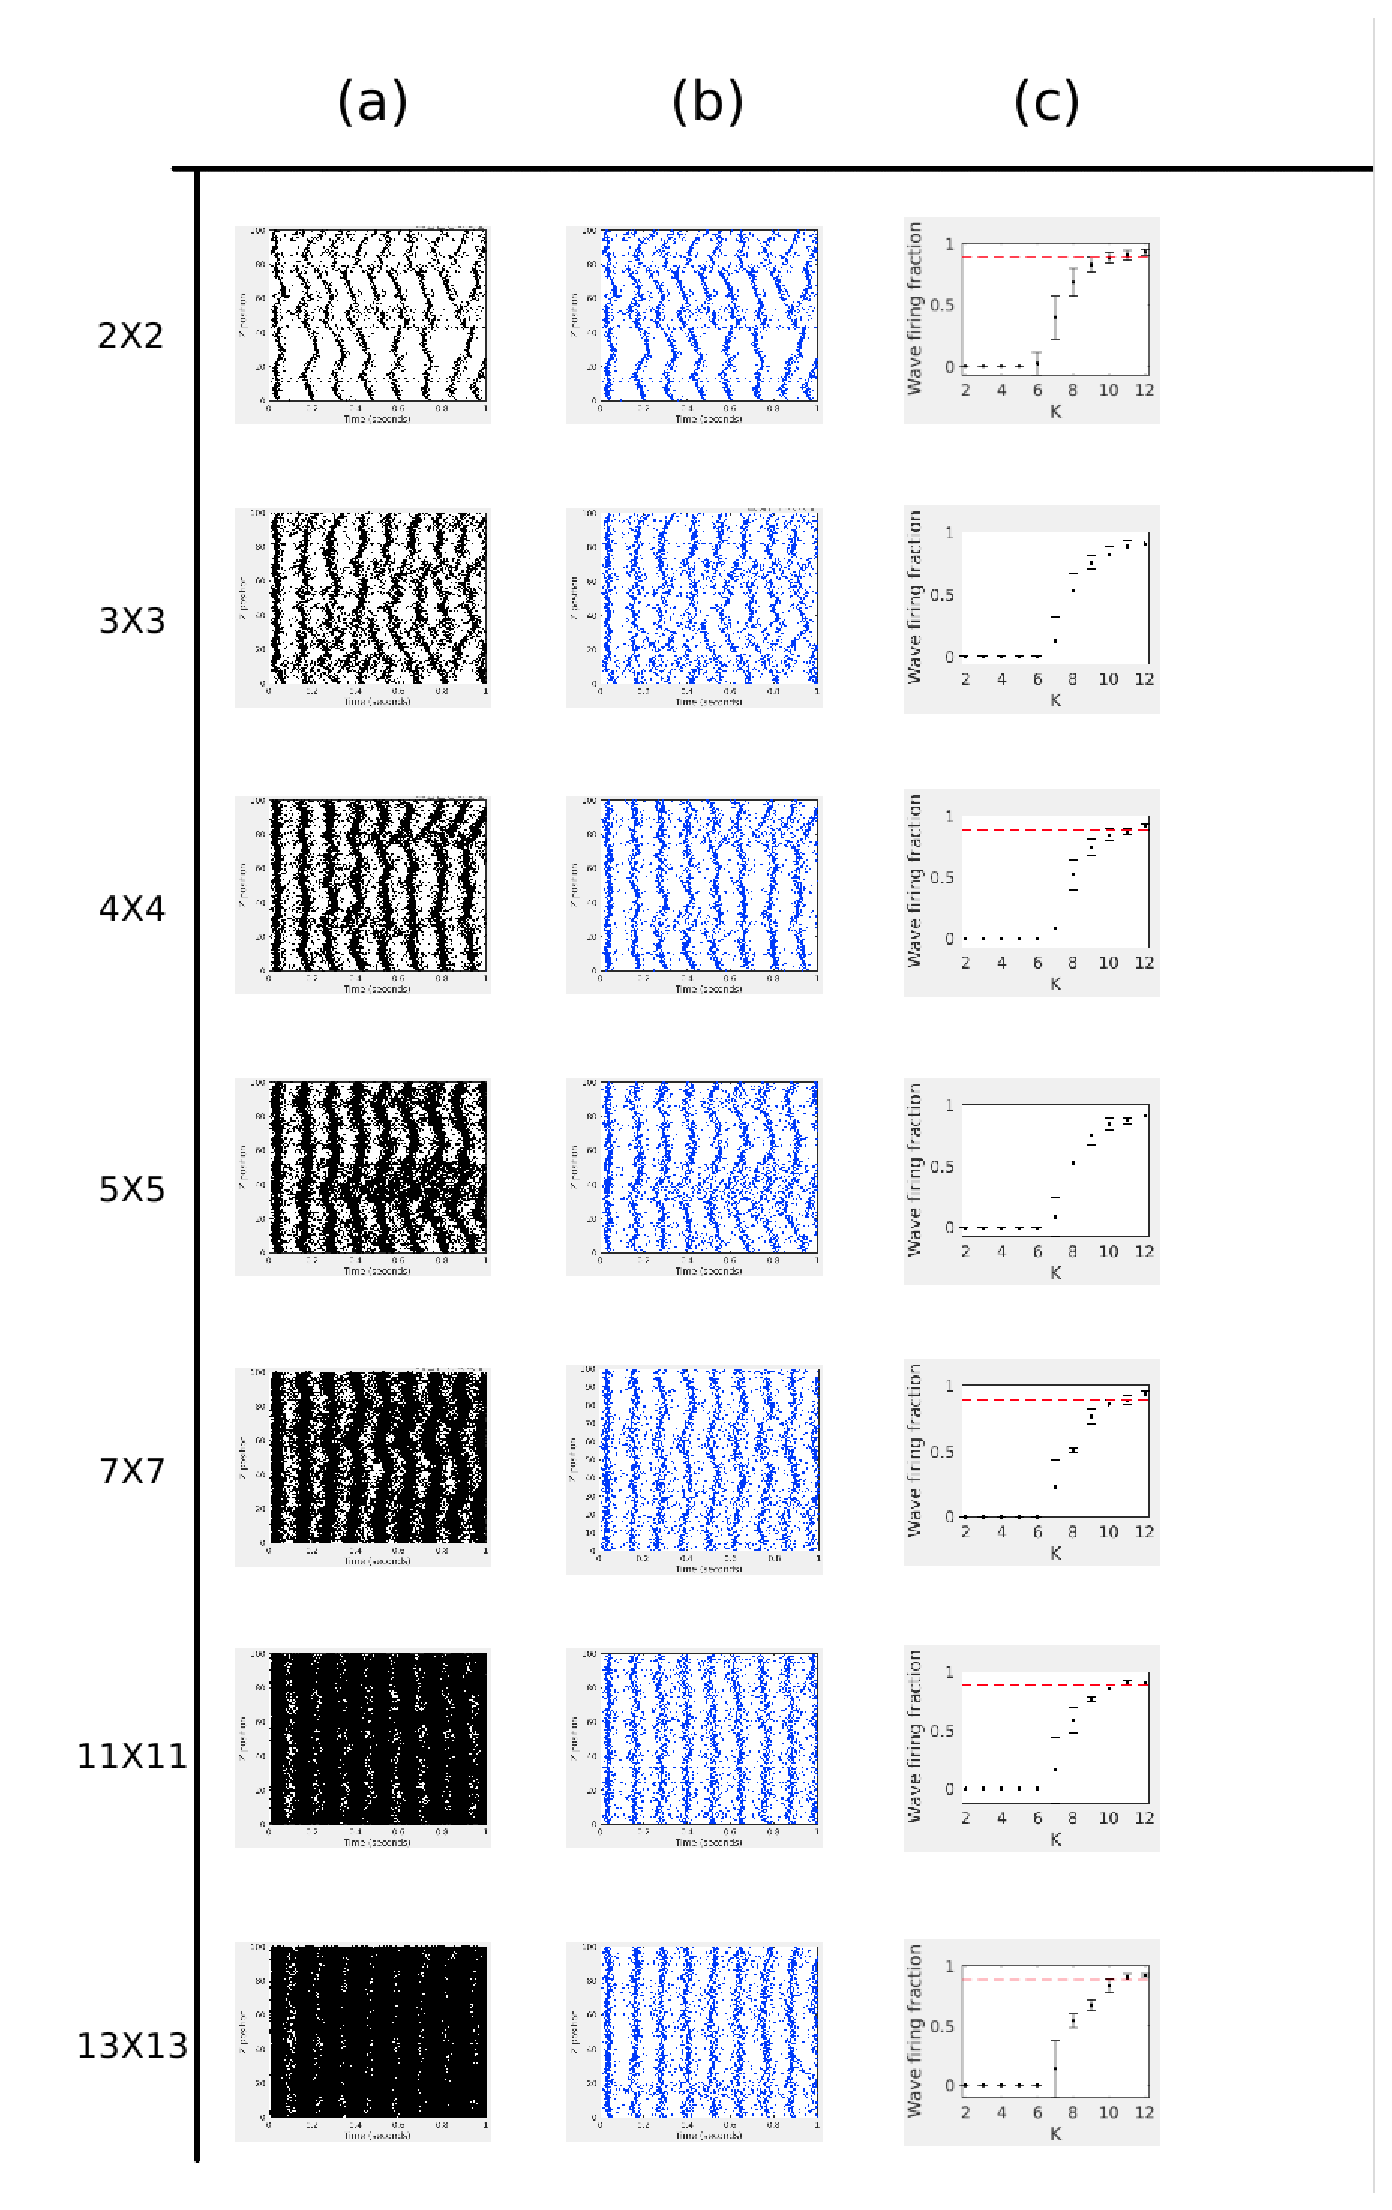
\includegraphics[width=0.75\textwidth]{fig/WaveFractionVsThick}
   \label{fig:LargeSCESubcolumns}
\end{figure}
\FloatBarrier

\section{Two-dimensional sheets of neurons}
\begin{figure}[!htb]
 \caption{ A two-dimensional sheet of neurons with connectivity according to Equation \ref{eq:connectivity}.}
 \label{fig:2D_connectivity}
 \centering
   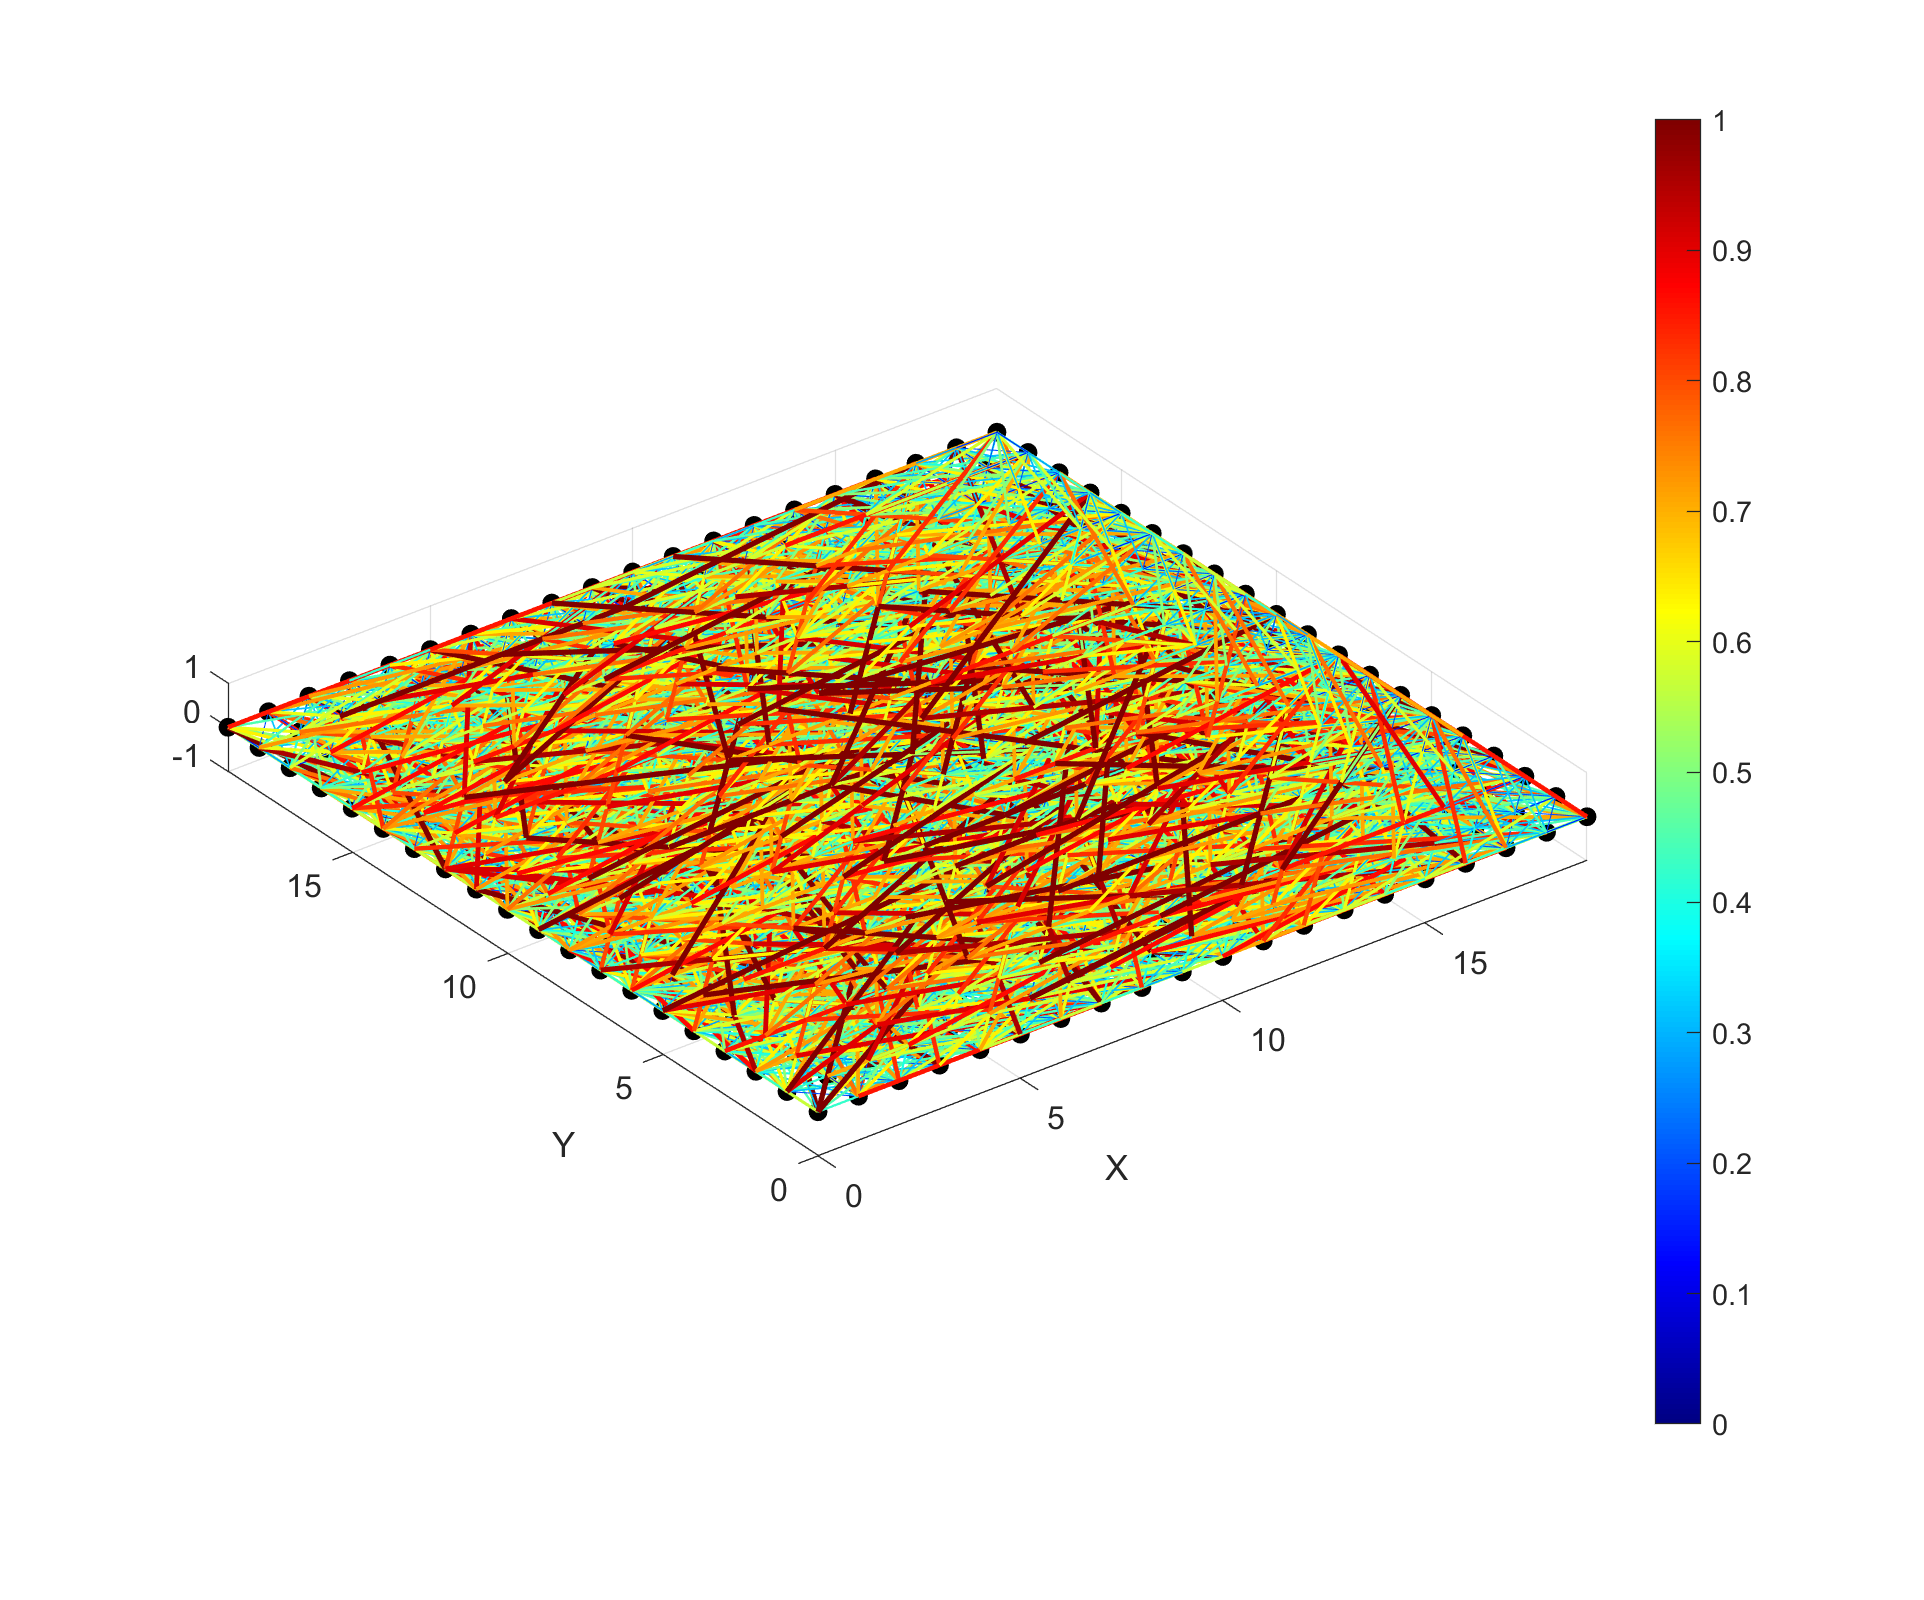
\includegraphics[width=\textwidth]{fig/2D_Connection_Plot}
\end{figure}

\FloatBarrier


\endinput
%%
%% End of file `example-1.tex'.
